\documentclass[12pt, twoside, openany]{report}
\usepackage[dvips]{graphicx,color,rotating}
\usepackage[utf8]{inputenc}
\usepackage{indentfirst}
\usepackage{t1enc}
\usepackage{a4wide}
\usepackage{amsfonts}
\usepackage{amsmath}
\usepackage{caption}
\usepackage{enumerate}
\usepackage{verbatim}
\usepackage[MeX]{polski}
\usepackage[T1]{fontenc}
\usepackage{geometry}
\geometry{left=25mm,right=25mm,bindingoffset=10mm, top=25mm, bottom=25mm}
\usepackage{amssymb, latexsym}
\usepackage{amsthm}
\usepackage{palatino}
\usepackage{float}
\usepackage{tabulary}
\usepackage{array}
\usepackage{pstricks}
\usepackage{textcomp}
\usepackage{url}
\usepackage{listings}
\usepackage{xcolor}
\usepackage{courier}
\usepackage{pgfplots}
\usepackage{etoolbox}
\patchcmd{\abstract}{\null\vfil}{}{}{} % abstract top align.

\newtheorem{twierdzenie}{Twierdzenie}[section]

%\linespread{1.5}

% styl listingów
\lstset{
mathescape,
    xleftmargin=17pt,
    numbers = left,
    %framexleftmargin=10mm,
    frame=lrbt,
    %backgroundcolor=\color[RGB]{250,250,250},
    %keywordstyle=\bfseries\color{blue},
    %identifierstyle=\bfseries,
    %numberstyle=\color[RGB]{0,192,192},
    %commentstyle=\it\color[RGB]{96,96,96},
    %stringstyle=\rmfamily\slshape\color[RGB]{128,0,0},
    %showstringspaces=true,
    breaklines=true,
    breakatwhitespace=try,
    %language=C++,
    showstringspaces=false,
    tabsize=4,
    basicstyle=\footnotesize\ttfamily,
    aboveskip=1em,
    %alsoletter={.},
    %morekeywords={n.find_successor, n.closest_preceding_node} % bolded keywords
    %postbreak=\raisebox{0ex}[0ex][0ex]{\ensuremath{\color{red}\hookrightarrow\space}}
}



\author{Mateusz Bartkowiak}
\title{Współbieżne modelowanie i~prezentacja dynamiki obiektów fizycznych}


\begin{document}

\begin{titlepage}

\noindent


\centering
\Large POLITECHNIKA POZNAŃSKA\\
\Large Wydział Informatyki\\
\large Systemy Rozproszone

\vfill

\includegraphics[width=120pt,height=120pt]{PP}

\vfill
\center
\LARGE
Mateusz Bartkowiak

\center
\Large
Praca magisterska

\vfill
\center
\Huge
\textbf{Efektywne wyszukiwanie danych w systemach P2P w oparciu o rozszerzenia protokołu Chord}


\vfill
\center
\Large
Promotor: dr inż. Anna Kobusińska

\vfill
\center
\large
Poznań, Październik 2018

\end{titlepage}

% wlasny abstract
\renewcommand{\abstractname}{}
\begin{abstract}
\thispagestyle{plain} % numer strony
\begin{center}
\textbf{Streszczenie}
\end{center}

\indent
Polskie streszczenie pracy.

\vspace{50px}
\begin{center}
\textbf{Abstract}
\end{center}

\indent
English abstract

\end{abstract}


\tableofcontents


%-----------Poczatek czesci zasadniczej-----------

\chapter{Wstęp}

\begin{itemize}
\item cel pracy i motywacja
\item zakres i omówienie rozdziałów
\end{itemize}


\chapter{Systemy Peer-to-Peer}

System P2P (ang. \textit{Peer-to-Peer}) jest z definicji systemem w którym wszystkie węzły tworzące sieć są równoważne w sensie funkcjonalnym i pełnią rolę zarówno klienta jak i serwera. Każdy węzeł może bezpośrednio nawiązywać połączenie z innym. Brak jest centralnego serwera który np. byłby głównym magazynem danych, bądź pośredniczyłby w komunikacji. Założenia te rodzą wiele problemów i ograniczeń, dlatego też budując komercyjne systemy P2P często odchodzi się od tej definicji wyróżniając specjalne węzły, które pełnią dodatkowe funkcje.

Rozdział ten pokazuje tło, na którym powstał protokół Statycznych Grup, wskazuje na pojawiające się problemy i wyzwania które należy podjąć, wskazuje istotność replikacji oraz opisuje różne budowy systemów P2P.

\section{Problemy i wyzwania}

Każdy system dużej skali stoi przed problemem awarii różnych części systemu. W odróżnieniu od wysoce niezawodnych centrów danych, systemy P2P często składają się z niepewnych węzłów, które nieraz pracują w niestabilnych warunkach (np. fizycznie poruszający się węzeł będący podłączony do sieci przez interfejs bezprzewodowy), czy dołączają do sieci tylko na pewien okres czasu. Zjawisko częstego rozłączania węzłów z sieci nazwijmy \textit{odpływem}. Natomiast zjawisko częstego dołączania węzłów do sieci nazwijmy \textit{przypływem}.

Systemy Peer-to-Peer są formą systemów rozproszonych z tą różnicą, że efekt odpływu jest w nich częstym i naturalnym zjawiskiem, co rodzi szereg dodatkowych problemów. Do tego dochodzą trudności typowe dla systemów rozproszonych, co razem sprawia, że skonstruowanie dobrego, w sensie poprawności i efektywności, systemu P2P jest zadaniem trudnym.

Dobry system P2P powinien spełniać szereg własności. Wybrane własności ważne z perspektywy zarządzania danymi są następujące:
\begin{itemize}
\item Dostępność: węzły powinny w każdym momencie mieć dostęp do potrzebnych danych.
\item Autonomia: węzły powinny móc dołączać i rozłączać się z sieci w każdej chwili, nie tworząc przy tym dodatkowych problemów, takich jak ograniczanie dostępności do danych.
\item Wydajność: system powinien efektywnie wykorzystywać dostępne zasoby sieci (przepustowość, moc obliczeniowa czy przechowywanie danych).
\item Jakość usług: z perspektywy użytkownika system powinien być wysokiej jakości, tzn. wyniki winne być kompletne, dane spójne i zawsze dostępne, a czas odpowiedzi powinien być krótki.
\item Odporność na awarie: ewentualne awarie, które się zdarzają, nie powinny mieć wpływu na wydajność, czy jakość usługi.
\item Bezpieczeństwo: naturalna otwartość systemów P2P sprawia, że bezpieczeństwo, głównie w kontekście nieuprawnionego dostępu do danych, jest dużym wyzwaniem.
\end{itemize}

\section{Replikacja}
\label{replikacja}

Remedium na problemy z dostępnością, jakością usług, czy odpornością na awarie powstałe w wyniku nieuniknionych odpływów, są mechanizmy replikacji. Po pierwsze, replikacja zwiększa dostępność poprzez eliminację pojedynczych punktów awarii (obiekty są dostępne z różnych węzłów). Po drugie, poprawia wydajność systemu poprzez redukcję obciążenia komunikacyjnego w sieci (obiekty mogą być umiejscowione bliżej węzłów pytających oraz są udostępniane jednocześnie z wielu węzłów). Ponadto replikacja poprawia skalowalność systemu, ponieważ przy wzroście liczby węzłów, możliwe jest zachowanie akceptowalnych czasów odpowiedzi.

Replikacja danych jest trudnym zagadnieniem, gdyż im wyższy stopień replikacji, tym wyższe koszty. Próby zminimalizowania kosztów w jednym obszarze, najczęściej kończą się podwyższeniem kosztów w innym. Poniżej przedstawione są trzy różne metryki kosztów związane z replikacją:
\begin{itemize}
\item Koszty monitoringu: potrzebne są mechanizmy monitoringu istniejących replik, aby mieć informację, czy są dostępne, oraz wychwytywanie nowych replik, aby móc zmienić lokalizację danych w przypadku awarii.
\item Koszty przesyłu danych: związane z tworzeniem nowych replik w systemie.
\item Koszty nierównomiernego obciążenia: niektóre mechanizmy replikacji mogą skutkować w nierównomiernej dystrybucji danych pomiędzy węzłami. Ma to znaczący wpływ na działanie systemu, ponieważ niektóre węzły mogą być przeciążone, podczas gdy inne będą nieużywane.
\end{itemize}

Jak zostało już nadmienione, poprawienie wszystkich powyższych metryk może okazać się niemożliwe. Dla przykładu, istnieją takie mechanizmy replikacji, które preferują replikowanie danych na węzłach bardziej niezawodnych. Pozwala to zaoszczędzić czas przesyłu danych (mniejsza częstotliwość tworzenia nowych replik), ale odbywa się to kosztem nierównomiernego obciążenia (bardziej niezawodne węzły będą bardziej obciążone). Ponadto twórcy konkretnych rozwiązań często badają swoje algorytmy pod kątem wybranych metryk, pomijając inne. Swoją drogą, analogiczną sytuację wskazuje tzw. teoria CAP, ukazująca spójność, dostępność i odporność na partycjonowanie jako trzy własności, których jednoczesne osiągnięcie jest niemożliwe.

W protokole Statycznych Grup intensywnie wykorzystywany jest mechanizm replikacji, aczkolwiek protokół ten abstrahuje od konkretnego sposobu replikowania, pozostawiając swobodę w tej kwestii.


\section{Sieć nakładkowa}
Systemy P2P wykorzystują do działania sieć nakładkową (ang. \textit{overlay network}), która jest dodatkową warstwą abstrakcji nadbudowaną nad istniejącą siecią (np. Internet). Parametry niefunkcjonalne systemu P2P takie jak odporność na awarie, autonomia węzłów, wydajność, skalowalność czy bezpieczeństwo zależą w dużej mierze od budowy sieci nakładkowej, którą można podzielić na trzy główne typy: nieustrukturyzowane, ustrukturyzowane oraz sieci z tzw. super-węzłami (ang. \textit{super-peer network}).

\subsection{Sieci nieustrukturyzowane}
\label{paragraf_sieci_ustrukturyzowane}
WW sieciach nieustrukturyzowanych, sieć nakładkowa jest budowana ad hoc w sposób niedeterministyczny. Rozmieszczenie danych jest zupełnie niezależne od topologii sieci nakładkowej, a każdy węzeł wie jedynie o swoich sąsiadach, aczkolwiek nie jest poinformowany o zasobach jakie posiadają. Mechanizmy wyszukiwania są z reguły proste, acz kosztowne. Przykładem może być mechanizm zalewania sieci zapytaniami o dany zasób, które krążą po sieci dopóki żądany zasób nie zostanie odnaleziony. Innym, nieco bardziej wyrafinowanym i wydajnym sposobem jest przesyłanie kilku równoległych zapytań, które każde jest przesyłane między węzłami w taki sposób, że jeden węzeł przesyła dalej zapytanie tylko do swojego jednego sąsiada. Z tego typu sieci nakładkowej korzystają m.in. takie systemy P2P jak Gnutella, Kazaa, czy FreeHaven. Jednym z największych wad sieci nieustrukturalizowanych jest niska skalowalności, gdyż przy coraz to większej ilości węzłów w sieci, znalezienie danego zasobu jest coraz bardziej kosztowne. Odpowiedzią na ten problem jest sieć ustrukturalizowana.

\subsection{Sieci ustrukturyzowane}
Sieci ustrukturyzowane charakteryzują się uzależnieniem lokalizacji danych od topologii sieci. Każdy zasób posiada swój identyfikator, który jednocześnie wskazuje miejsce w sieci, w którym się znajduje. Głównym reprezentantem tej klasy sieci są systemy DHT (ang. \textit{distributed hash table}). Systemy te udostępniają interfejs tablic mieszających, gdzie klucze są identyfikatorami obiektów. Każdy węzeł odpowiedzialny jest za przechowywanie tych danych, których wartość kluczy mieści się w odpowiednim dla niego, ściśle określonym zakresie. Ponadto każdy węzeł ma informacje o pewnej liczbie innych węzłów w sieci (sąsiadów): przechowuje tablice rutingu w której przypisane są identyfikatory sąsiadów do odpowiednich adresów. Większość operacji dostępu do danych to operacje \textit{lookup}, czyli próby znalezienia lokalizacji jakiegoś obiektu. Operacja lookup najczęściej wykorzystywana jest do znalezienia adresu węzła odpowiedzialnego za dany zasób, dzięki czemu węzeł pytający może bezpośrednio nawiązać z nim komunikację. Aby skutecznie odnaleźć węzeł odpowiedzialny, pojedyncze wywołanie tej operacji może skutkować kilkoma przeskokami żądania pomiędzy sąsiadami. Ponieważ każdy węzeł jest odpowiedzialny za pewien zakres kluczy oraz współtworzy system trasowania, autonomia pojedynczego węzła jest mocno ograniczona. Jest to największą wadą sieci ustrukturalizowanych, gdyż każde dołączenie, bądź rozłączenie węzła zaburza strukturę sieci, co skutkuje potrzebą przeprowadzenia jej rekonstrukcji. Przykładami tego typu sieci są takie systemy jak Chord (więcej o protokole Chord w rozdziale \ref{rozdzial_chord}), CAN, Tapestry, Pastry, Pier, OceanStore, czy Past. Protokół Statycznych Grup opiera się na rozszerzeniu protokołu Chord, a więc intensywnie korzysta zalet sieci ustrukturalizowanych klasy DHT, lecz i cierpi z powodu wyżej wymienionych wad.

\subsection{Sieci z super-węzłem}
W sieciach ustrukturalizowanych oraz nieustrukturalizowanych wszystkie węzły są takie same pod względem funkcjonalności. Inaczej się ma sprawa z sieciami super-peer (sieci z super-węzłami), które stanowią klasę pośrednią, między modelem P2P a modelem klient-serwer. W sieciach tej klasy niektóre węzły pełnią specjalne role w sieci, spełniając takie dodatkowe funkcje jak indeksowanie, przetwarzanie zapytań, kontrola dostępu, czy zarządzanie metadanymi. W przypadku awarii, rolę super-węzłów mogą dynamicznie przejmować inne węzły. Działanie tych sieci przeważnie polega na wysyłaniu zapytań do super-węzła, który posiada informacje o położeniu żądanych obiektów. Dlatego też zaletami sieci super-peer są wydajność oraz jakość usługi. Czas potrzebny na znalezienie żądanego obiektu jest zazwyczaj krótszy, niż w przypadku zalewania sieci. Ponadto heterogeniczność węzłów w sensie ich zasobów i wydajności można wykorzystać do wyróżnionych zadań, obierając je za super-węzły. Jednakże autonomia węzłów w owych sieciach jest ograniczona, a odporność na awarie jest niska, gdyż super-węzły stają się pojedynczymi punktami awarii (skutki tego problemu można załagodzić dynamicznie wybierając nowe super-węzły). Z tego typu sieci korzystają m.in. takie systemy jak Napster, Publius, Edutella, czy JXTA.


\chapter{Protokół Chord}
\label{rozdzial_chord}

%jak dziala
%pseudokod

%rozproszony protokół do wyznaczania lokalizacji danego obiektu (wspomniana w paragrafie \ref{paragraf_sieci_ustrukturyzowane} operacja lookup)
%istniejące rozszerzenia

Fundamentalnym problemem z którym należy się zmierzyć tworząc system P2P jest efektywne znalezienie węzła odpowiedzialnego za dany zasób. Rozdział ten przedstawia protokół, który jest odpowiedzią na ten problem i na podstawie którego zbudowano protokół Statycznych Grup: Chord, rozproszony protokół do zidentyfikowania lokalizacji danego obiektu. Chord dostarcza operację wyznaczenia węzła na podstawie klucza. Dzięki temu można odnaleźć żądany zasób (który jest reprezentowany przez odpowiedni klucz). Chord dostosowywuje się do dynamicznego dołączania oraz rozłączania węzłów z systemu, i nawet podczas tych zmian systemu działa w prawidłowy sposób, zachowując przy tym dobrą skalowalność.

%Chord wspiera tylko i aż jedną operację \textit{lookup}, która mapuje klucz na węzeł. W zależności od aplikacji używającej Chorda, węzeł mógłby np. być odpowiedzialny za przechowywanie wartości związanej z danym kluczem. Chord do przypisywania kluczy węzłom, używa mieszania spójnego (ang. \textit{consistent hashing}). Mieszanie te wpływa na równomierne obciążenie, gdyż każdy węzeł otrzymuje podobną liczbę kluczy.
%Każdy węzeł potrzebuje mieć informacje tylko o paru węzłach, aby móc dobrze działać. Dzięki temu zachowana jest skalowalność. Ponieważ informacje potrzebne do trasowania są rozproszone między węzłami, podczas wykonywania operacji lookup, węzeł komunikuje się z innymi. Każdy węzeł przechowuje informacje o $\mathcal{O}(\log{}N)$ innych węzłach. Złożoność komunikacyjna operacji lookup również wynosi $\mathcal{O}(\log{}N)$. Jednakże podczas dużego odpływu, gdy informacje potrzebne do trasowania są nieaktualne, efektywność spada znacząco.


\section{Opis}
Chord wspiera tylko i aż jedną operację \textit{lookup}, która mapuje klucz na węzeł. Upraszcza konstrukcję systemu P2P i aplikacji bazującej na nim zapewniając następujące własności:

\begin{itemize}
\item Równowaga obciążenia: Chord działa jak rozproszona funkcja mieszająca, równomiernie rozpraszając klucze po węzłach.

\item Decentralizacja: Chord działa w rozproszeniu i żaden węzeł nie jest ważniejszy od innego.

\item Skalowalność: koszt operacji lookup rośnie logarytmicznie wraz z wzrostem liczby węzłów, dlatego też działa sprawnie nawet w systemach z relatywnie dużą liczebnością węzłów.

\item Dostępność: Chord automatycznie dostraja się do ciągłych zmian w sieci, zapewniając, że węzeł odpowiedzialny za dany klucz może w każdej chwili zostać odnaleziony.

\item Elastyczne nazewnictwo: Chord nie wymusza struktury nazewniczej kluczy - przestrzeń kluczy jest płaska. Aplikacja korzystająca z tego protokołu ma dużą swobodę w sposobie mapowania własnych nazw na klucze.
\end{itemize}

W kontekście budowania aplikacji, o Chordzie można myśleć jak o bibliotece, która dostarcza tej aplikacji operację \texttt{lookup(key)}, oraz powiadamia ją na danym węźle o zmianie zbioru kluczy, za które ten węzeł jest odpowiedzialny. Dzięki temu, aplikacja może podjąć stosowne działania, jak np. przenieść odpowiednie wartości do nowo dołączonego węzła. Aplikacja używająca Chorda jest odpowiedzialna za ewentualną autentykację, używanie pamięci podręcznej, replikację, czy przyjazne dla użytkownika nazewnictwo danych. Płaska przestrzeń
adresowa ułatwia implementację tych funkcjonalności. Dla przykładu, aplikacja mogłaby autentykować dane, przechowując je pod kluczem pochodzącym z mechanizmów kryptograficznych. Tak samo, aplikacja mogłaby replikować dane poprzez przechowywanie ich na miejscach związanych z kluczami wywiedzionymi z identyfikatora tych danych z poziomu aplikacji.


\section{Protokół}

Protokół Chord określa jak odnaleźć lokalizację kluczy, jak nowe węzły są dołączane do systemu oraz jak poradzić sobie z odłączaniem węzłów (planowanym bądź nie).

\subsection{Identyfikatory}

Funkcja spójnego mieszania (ang. \textit{consistent hash function}) przypisuje każdemu węzłowi oraz kluczowi \textit{m}-bitowy identyfikator. Identyfikator węzła generowany jest z jego adresu IP, a identyfikator klucza bezpośrednio z wartości. Długość identyfikatora \textit{m} musi być odpowiednio duża, aby zapewnić jak największą odporność na kolizje.

Identyfikatory są ułożone kolejno według wartości na \textit{okręgu identyfikatorów}. Okrąg ten, z numerami od $0$ do  $2^m-1$ , będziemy nazywać \textit{pierścieniem}. Klucze są przypisane temu węzłowi, którego identyfikator znajduje się na okręgu jako pierwszy po danym kluczu \textit{k}, lub jest jemu równy. Ten węzeł nazywa się \textit{następnikiem} klucza \textit{k} i oznaczany jest jako \texttt{successor(k)}. Przykładowy pierścień pokazany jest na rysunku \ref{fig:pierscien}.

\begin{figure}[H]
\floatstyle{boxed}
\centering
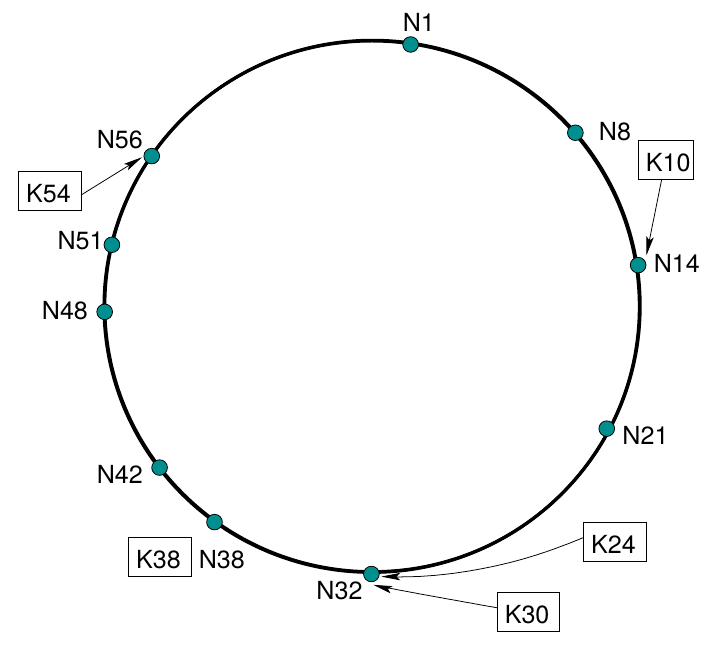
\includegraphics[width=0.6\textwidth,height=\textheight,keepaspectratio]{ring.png}
\caption{Okrąg identyfikatorów (pierścień) zawierający dziesięć węzłów, które przechowują w sumie pięć kluczy.}
\label{fig:pierscien}
\end{figure}

Utrzymywanie pierścienia odbywa się w następujący sposób: gdy węzeł \textit{n} dołączy do sieci, odpowiednie klucze, poprzednio przypisane następnikowi węzła \textit{n}, zostają przypisane do \textit{n}. Kiedy węzeł \textit{n} opuści sieć, wszystkie klucze za które był odpowiedzialny są przypisane na nowo do następnika \textit{n}. Dla przykładu, jeśli do sieci reprezentowanej przez pierścień na rysunku \ref{fig:pierscien} dołączyłby węzeł o identyfikatorze 26, to klucz 24 zostałby przeniesiony z węzła 32 do nowo dołączonego węzła.

\subsection{Odnajdywanie lokalizacji klucza}

Każdy węzeł posiada wskaźnik na swojego następnika. Dzięki temu w prosty sposób możliwe jest odnalezienie węzła odpowiedzialnego za dany klucz poprzez rekurencyjne odpytywanie się kolejnych następników. Posiadanie aktualnego wskaźnika na swojego następnika jest warunkiem koniecznym otrzymania poprawnego wyniku. Aczkolwiek aby zmniejszyć liczbę komunikatów podczas operacji lookup, każdy węzeł posiada dodatkowe informacje trasowania. Informacje te przechowywanie są w specjalnej tablicy trasowania, którą określa się mianem \textit{finger table}. Niech \textit{m} będzie liczbą bitów używanych do zapisywania identyfikatorów kluczy i węzłów. Wtenczas tablica trasowania posiada \textit{m} wpisów. Każdy \textit{i}-ty wpis tej tablicy węzła \textit{n} posiada informacje o pierwszym węźle \textit{s} (jego identyfikator oraz adres, który służy do komunikacji - jest nim najczęściej adres IP), który jest za \textit{n} o przynajmniej $2^{i-1}$ na okręgu identyfikatorów. Wzór na identyfikator węzła \textit{s} w \textit{i}-tym wpisie węzła \textit{n}, gdzie $1\leq i \leq m$:

\begin{equation}
\label{eq:start}
s=successor(n+2^{i-1})
\end{equation}

Warto zwrócić uwagę, że pierwszy wpis w tablicy trasowania węzła \textit{n} jest jego bezpośrednim następnikiem na pierścieniu. Na rysunku \ref{fig:finger_table} pokazane są wpisy w tablicy trasowania węzła 8. Pierwszy wpis wskazuje na węzeł 14, gdyż jest on pierwszym węzłem który jest przed wartością $(8+2^0) \bmod 2^6=9$. Podobnie, ostatni wpis wskazuje na węzeł 42, ponieważ jest on pierwszym węzłem, który jest przed wartością $(8+2^5) \bmod 2^6=40$.

\begin{figure}[H]
\floatstyle{boxed}
\centering
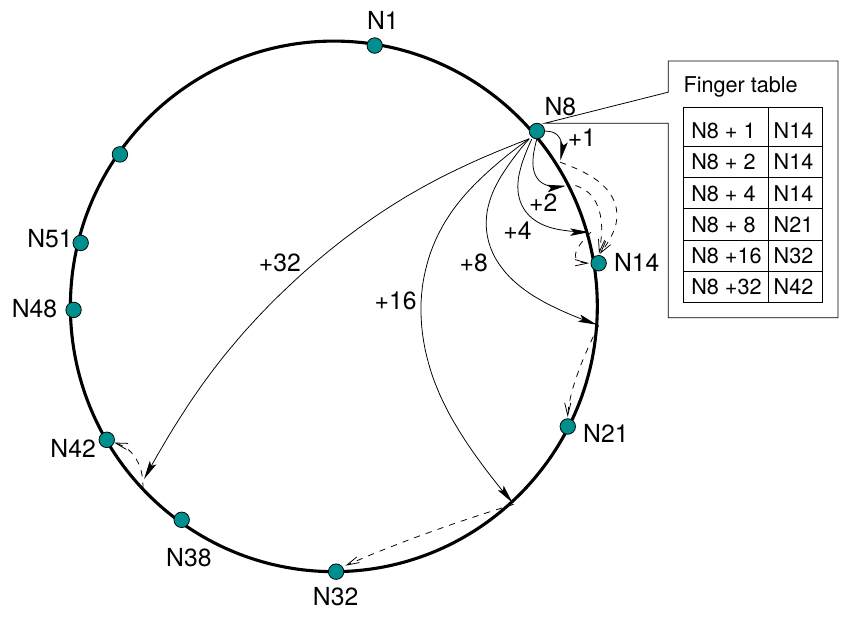
\includegraphics[width=0.8\textwidth,height=\textheight,keepaspectratio]{finger_table.png}
\caption{Wpisy tablicy trasowania węzła 8.}
\label{fig:finger_table}
\end{figure}

Schemat ten posiada dwie cechy. Po pierwsze, każdy węzeł posiada informację o małej liczbie węzłów, z czego większość tych węzłów znajduje się w małej odległości od niego na pierścieniu. Po drugie, korzystając z tablicy trasowania z reguły nie można bezpośrednio określić następnika dowolnego klucza. Dla przykładu, węzeł 8 na rysunku \ref{fig:finger_table} nie może samodzielnie ustalić bezpośredniego następnika klucza 34, gdyż następnik ten (węzeł 38) nie znajduje się w tablicy trasowania węzła 8.

Listing \ref{lst:find_successor} pokazuje pseudokod funkcji \textit{find\_successor}, która jest odpowiednikiem operacji lookup, czyli odnalezienia węzła odpowiedzialnego za dany klucz. Jeżeli identyfikator \textit{id} znajduje się pomiędzy identyfikatorem aktualnego węzła \textit{n} a identyfikatorem następnika \textit{successor} tego węzła, to funkcja ta zwraca wskaźnik na następnik węzła \textit{n}. W przeciwnym wypadku, wykorzystując funkcję \textit{closest\_preceding\_node} pokazaną na listingu \ref{lst:closest_preceding_node}, węzeł \textit{n} przeszukuje tablice trasowania, aby znaleźć taki węzeł \textit{n'}, którego identyfikator jest najbliższy lecz mniejszy od \textit{id}; i następnie wywołuje zdalną metodę \textit{find\_succesor} węzła \textit{n'}. Wybieranie węzła \textit{n'} odbywa się w taki sposób, ponieważ im węzeł znajduje się bliżej \textit{id} na pierścieniu, tym posiada więcej informacji o obszarze pierścienia wokół \textit{id}.

\lstinputlisting[caption={Pseudokod funkcji odpowiedzialnej za znalezienie następnika obiektu o danym identyfikatorze.}, captionpos=b, label={lst:find_successor}, float=h]{find_successor.txt}

\lstinputlisting[caption={Pseudokod funkcji odpowiedzialnej za znalezienie najwyższego poprzednika obiektu o danym identyfikatorze z tablicy trasowania.}, captionpos=b, label={lst:closest_preceding_node}, float=h]{closest_preceding_node.txt}

\begin{figure}[H]
\floatstyle{boxed}
\centering
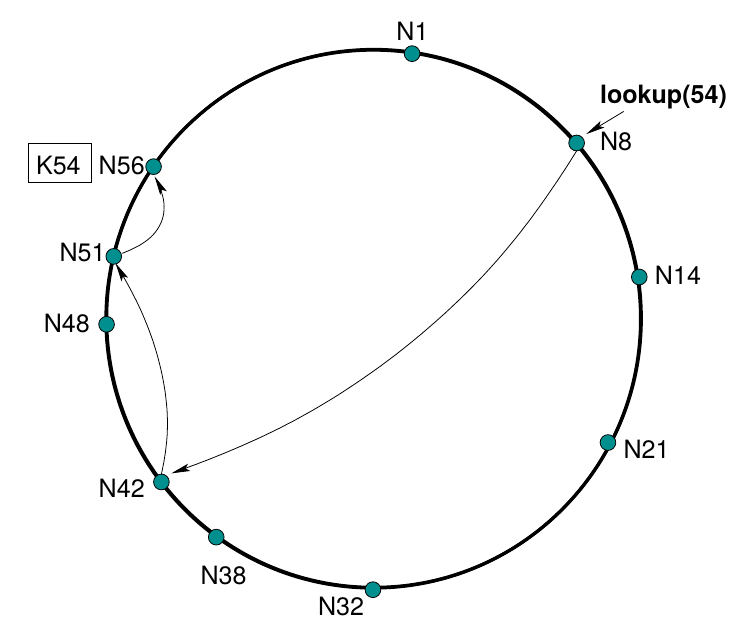
\includegraphics[width=0.6\textwidth,height=\textheight,keepaspectratio]{lookup_example.png}
\caption{Ścieżka zapytania o klucz 54 rozpoczynającego się od operacji lookup węzła 8.}
\label{fig:lookup_example}
\end{figure}

Przykładowo węzeł 8 chciałby znaleźć następnika klucza 54. Sytuacja ta pokazana jest na rysunku \ref{fig:lookup_example}. Ponieważ ostatnim wpisem w tablicy trasowania węzła 8, który poprzedza 54, jest węzeł 42, to węzeł 8 wyśle zapytanie do węzła 42. Dalej, węzeł 42 przeszuka swoją tablicę trasowania, aby odnaleźć największy węzeł, który poprzedza klucz 54, i będzie to węzeł 51. Wyśle więc do niego zapytanie, a węzeł 51 odpowie, że to jego następnik, węzeł 56, jest następnikiem klucza 54. Ostatecznie odpowiedź ta wróci do węzła 8.

Twórcy protokołu Chord udowadniają \cite{bib:chord}, iż złożoność komunikacyjna operacji lookup, w sieci składającej się z \textit{N} węzłów, z dużym prawdopodobieństwem wynosi $\mathcal{O}(\log{}N)$. A średni czas odnalezienia węzła odpowiedzialnego za dany klucz podczas eksperymentów wyniósł $\frac{1}{2} \log{} N$.

\subsection{Zmiany w sieci}

W praktyce, Chord musi radzić sobie z ciągłym dołączaniem węzłów oraz ich nieprzewidywalnym odłączaniem. Aby operacja lookup zawsze zwracała poprawny wynik mimo zmian w sieci, protokół Chord musi zapewnić, aby w każdym węźle wskaźniki na następnika były aktualne. Dbają o to specjalne procedury wykonywane cyklicznie przez wszystkie węzły, które uaktualniają tablice trasowania oraz wskaźniki na następnika i poprzednika. 

Pseudokod procedury odpowiedzialnej za dołączanie węzła pokazuje listing \ref{lst:join}. Węzeł \textit{n} dołącza się do istniejącego pierścienia przy pomocy innego węzła \textit{n'}, który tworzy owy pierścień. Jeżeli jednak węzeł \textit{n} ma zamiar stworzyć nowy pierścień, wywołuje procedurę \textit{create} pokazaną na listingu \ref{lst:create}. Samo dołączenie do sieci nie sprawia, iż reszta węzłów w sieci wie o nowym węźle. Dopiero procedura stabilizacji \textit{stabilize}, pokazana na listingu \ref{lst:stabilize} i uruchamiana cyklicznie przez każdy węzeł, uaktualnia informacje o węzłach w sieci. Za każdym razem, gdy węzeł \textit{n} uruchomi stabilizację, sprawdzane jest czy to poprzednik \textit{p} następnika \textit{successor} węzła \textit{n} nie powinien być jego następnikiem. Będzie tak, jeśli \textit{p} jest nowo dołączonym węzłem. Dodatkowo, wywołując procedurę \textit{notify} pokazaną na listingu \ref{lst:notify}, stabilizacja powiadamia następnika węzła \textit{n} o istnieniu węzła \textit{n} w sieci, dając szansę na uaktualnienie wskaźnika na poprzednika.


\lstinputlisting[caption={Pseudokod procedury odpowiedzialnej za utworzenie nowego pierścienia Chord.}, captionpos=b, label={lst:create}, float=!h]{create.txt}

\lstinputlisting[caption={Pseudokod procedury odpowiedzialnej dołączenie węzła do pierścienia Chord zawierającego węzeł \textit{n'}.}, captionpos=b, label={lst:join}, float=!h]{join.txt}

\lstinputlisting[caption={Pseudokod procedury wywoływanej okresowo i odpowiedzialnej za weryfikację bezpośredniego następnika \textit{successor} węzła \textit{n} oraz powiadomienie go o \textit{n}.}, captionpos=b, label={lst:stabilize}, float=!h]{stabilize.txt}

\lstinputlisting[caption={Pseudokod procedury odpowiedzialnej za ewentualną aktualizację wskaźnika na poprzednika \textit{predecessor}.}, captionpos=b, label={lst:notify}, float=!h]{notify.txt}

\lstinputlisting[caption={Pseudokod procedury wywoływanej okresowo i odpowiedzialnej za aktualizację wpisów w tablicy trasowania.}, captionpos=b, label={lst:fix_fingers}, float=!h]{fix_fingers.txt}

\lstinputlisting[caption={Pseudokod procedury wywoływanej okresowo i odpowiedzialnej za wyzerowanie wskaźnika na poprzednika \textit{predecessor} w przypadku jego awarii.}, captionpos=b, label={lst:check_predecessor}, float=!h]{check_predecessor.txt}

Każdy węzeł okresowo uruchamia procedurę \textit{fix\_fingers} pokazaną na listingu \ref{lst:fix_fingers}, która uaktualnia wpisy w tablicy trasowania. Dzięki temu nowe węzły wypełniają swoje tablice, a węzły będące wcześniej w sieci, aktualizują je o ewentualne nowe węzły. Ponadto każdy węzeł wykonuje cyklicznie procedurę \textit{check\_predecessor} pokazaną na listingu \ref{lst:check_predecessor}, która zeruje wskaźnik na poprzednika, jeśli uległ on awarii. Wskaźniki te uaktualniane są podczas cyklicznej operacji \textit{notify}.

W praktyce, przez ciągłe przypływy oraz odpływy węzłów, stan pierścienia Chord nigdy nie będzie stabilny. Dołączenia, rozłączenia i cykliczny algorytm stabilizacji będą się przeplatały bez końca. Pierścień nie będzie miał czasu, aby ustabilizować się w pełni, nim nastąpi zmiana w zbiorze węzłów sieci. Jednakże autorzy protokołu zapewniają, że jeśli protokół stabilizacji będzie uruchamiany z odpowiednią częstotliwością, to pierścień będzie utrzymywał się w stanie ,,prawie stabilnym'', w którym to operacje lookup wykonują się sprawnie i zwracają poprawne wyniki \cite{bib:chord}.

\section{Istniejące rozszerzenia}

Protokół Chord jest prosty w swojej idei. Jego konstrukcja pozostawia duże pole do ewentualnych rozszerzeń. Sami autorzy zaproponowali kilka prostych usprawnień. Ponadto powstało wiele pomysłów jak rozszerzyć Chorda o dodatkowe funkcjonalności, takie jak replikacja danych. Są też rozwiązania, które korzystają z Chorda, dostosowywując go do swoich potrzeb. Sam motyw przewodni tej pracy bazuje na rozszerzeniu protokołu Chordzie o dodatkowy mechanizm grupowania.

\subsection{Usprawnienie działania}

Aby poprawić działanie protokołu Chord, autorzy proponują dwa rozszerzenia. Po pierwsze, zamiast wskaźnika na następnika, każdy węzeł może utrzymywać listę następników. Dzięki temu mógłby odwołać się do innego następnika, jeżeli bliższy następnik uległ awarii. Poprawia to działanie protokołu, gdyż uodparnia na odpływy, zachowując wydajność operacji lookup na wysokim poziomie. Drugą rekomendacją autorów jest zaimplementowanie procedury odłączenia z sieci. W bazowej implementacji odejście węzła polega na jego nagłym rozłączeniu, bez informowania sieci i traktuje się je tak jak awarie. Zamiast tego, węzeł mógłby poinformować swojego następnika oraz poprzednika, że opuszcza sieć, dzięki czemu mogłyby one uaktualnić wskaźniki. Ponadto węzeł mógłby przed opuszczeniem przetransferować klucze za które jest odpowiedzialny, swojemu następnikowi. Zamiany ta zwiększyłyby dostępność systemu, oraz poprawiły jego wydajność.

\subsection{Replikacja}

Jak zostało wspomniane w podrozdziale \ref{replikacja}, replikacja danych zwiększa dostępność systemu. W protokole Chord nie występuje natywnie owy mechanizm, dlatego też podczas awarii węzła, wszystkie klucze, za które odpowiadał, zostają utracone, stając się niedostępnymi. Są zastosowania, w których ,,problem'' ten problemem nie będzie. Lecz są i takie systemy, w których replikacja jest konieczna.

Najprostszym rozwiązaniem wydaje się być replikacja u sąsiadów (ang. \textit{Neighbor Replication}). W podejściu tym, każdy węzeł dba, aby dane replikować u swoich sąsiadów. Mechanizm ten jest elastyczny, gdyż pozwala indywidualnie (osobno przez każdy węzeł) kontrolować stopień replikacji, dzięki czemu można dobierać odpowiednie polityki według potrzeb; np. replikować popularne dane\footnote{Dane popularne to te, o które relatywnie często przychodzą żądania.} na bardziej stabilnych węzłach, bądź na większej ich ilości. Zaletą tego podejścia są niskie koszty monitoringu. Wadą natomiast wysokie koszty utrzymywania replik.

Innym podejściem jest tzw. multi-publikacja (ang. \textit{Multi-Publication}). Rozwiązanie te opiera się na replikowaniu danych na wielu, deterministycznie wyznaczonych pozycjach w pierścieniu Chord. Sposób wyznaczania pozycji może być dowolny, aczkolwiek jest stały dla całej sieci, a więc o wiele mniej elastyczny, niż replikacja u sąsiadów. Sugerowane jest, aby obiekt był przechowywany pod wieloma kluczami, które wyznaczane są kilkoma funkcjami skrótu. Problemem multi-publikacji są odpływy, które trzeba monitorować, aby zachować ustalony stopień replikacji. Natomiast plusem może być dobre zrównoważenie obciążenia (w zależności od doboru metody wyznaczania pozycji).

\subsection{Inne}

Istnieje też wiele innych rozwiązań mających u swego rdzenia mechanizm Chord. Dobrym przykładem jest algorytm TAC (ang. Topology Aware Chord)\cite{bib:tac}, rozszerzający Chorda o mechanizmy kontrolujące topologię sieci nakładkowej w zależności od fizycznej sieci w której działa. Autorzy twierdzą, że dzięki temu uzyskali lepszą wydajność pod kątem trasowania wiadomości oraz zużycia pasma.

Chord został tak zaprojektowany, aby rozszerzanie go nie stanowiło problemu. Dlatego powstało wiele pomysłów jak go zmienić, aby poprawić różne parametry systemu. Sam Protokół Statycznych Grup, jest w swojej istocie rozszerzeniem Chorda, ale ponieważ jest on tematem przewodnim tej pracy, został mu poświęcony osobny rozdział (\ref{rozdzial_rozwiazanie}).


\chapter{Grupowanie węzłów}
\label{rozdzial_grupowanie}
\begin{itemize}
\item idea
\item istniejące rozwiązania
\end{itemize}




\chapter{Zaproponowane rozwiązanie}
\label{rozdzial_rozwiazanie}
\begin{itemize}
\item ogolny opis
\item do czego dążę
\item od czego abstrachuję
\item szczegolowy opis, pseudokod
\end{itemize}


\chapter{Testy symulacyjne}

\begin{itemize}
\item opisac PeerSim
\item scenariusze: ile wezlow, jak czesto dolaczaja, jak duze sa grupy, wspolczyniki stabilizacji
\item wyniki
\item analiza
\end{itemize}


\chapter{Podsumowanie}

\begin{itemize}
\item o czym byla praca, czy cel osiagniety, czy spoko wyniki, dalsze rozwiazania
\end{itemize}


%-----------Koniec czesci zasadniczej-----------


\begin{thebibliography}{11}
\addcontentsline{toc}{chapter}{Bibliografia} % dodane do spisu treści

\bibitem{bib:martins} Vidal Martins, \emph{Data Replication in P2P Systems}, Réseaux et télécommunications [cs.NI], Université de Nantes, 2007, Français

\bibitem{bib:jeyasheeli} Ms. F. Golda Jeyasheeli, L. Rajashree, \emph{Cost Effective File Replication in P2P File Sharing Systems}, 2012 International Conference on Computing, Electronics and Electrical Technologies [ICCEET]
 
\bibitem{bib:ye} C. Ye, D. M. Chiu, \emph{Peer-to-Peer Replication with Preferences}, Department of Information Engineering, The Chinese University of Hong Kong

\bibitem{bib:paiva} J. Paiva, L. Rodrigues, \emph{Policies for Efficient Data Replication in P2P Systems}, INESC-ID, Instituto Superior Técnico, Universidade Técnica

\bibitem{bib:kobusinska} Anna Kobusińska, \emph{Systemy Rozprosozne Dużej Skali}, Wykłady, 2017, Instytut Informatyki, Politechnika Poznańska

\bibitem{bib:chord}  I. Stoica, R. Morris, D. Liben-Nowell, D. R. Karger, M. F. Kaashoek, F. Dabek, and H. Balakrishnan, \emph{Chord: A Scalable Peer-to-Peer Lookup Protocol for Internet Applications}, MIT Laboratory for Computer Science

\bibitem{bib:chord_lec} Smruti R. Sarangi, \emph{Distributed Hash Tables, Chord}, Lectures, Department of Computer Science, Indian Institute of Technology, New Delhi, India

\bibitem{bib:chord_lec} P. Knezevic, A. Wombacher, T. Risse, \emph{Enabling High Data Availability in a DHT}, 16th International Workshop on Database and Expert Systems Applications, 2005 (pp. 363-367). [10.1109/DEXA.2005.84] Los Alamitos: IEEE Computer Society Press. DOI: 10.1109/DEXA.2005.84

\bibitem{bib:chord_lec} A. Rao, K. Lakshminarayanan, S. Surana, R. Karp, I. Stoica, \emph{Load Balancing in Structured P2P Systems}, Peer-to-Peer Systems II. IPTPS 2003. Lecture Notes in Computer Science, vol 2735. Springer, Berlin, Heidelberg

\bibitem{bib:tac} Javad Taheri , Mohammad Kazem Akbari, \emph{TAC: A Topology-Aware Chord-based Peer-to-Peer Network}, Advanced Information Technologies Lab., Department of Computer Engineering and IT, Amirkabir University of Technology, Tehran, Iran

%\bibitem{bib:kobusinska} Anna Kobusińska, \emph{Systemy Rozprosozne Dużej Skali}, Wykłady, [online] \url{http://www.cs.put.poznan.pl/akobusinska/lsds.html} [dostęp: 23.08.2018 r.]

\end{thebibliography}

\end{document}
